\section{Introduction}

The core idea of this project is to use the Haskell type system to automatically derive succinct, almost information-theoretically optimal runtime representations for standard algebraic data types (products and sums) and common built-in types such as \texttt{Int} and \texttt{Bool}. In functional programming, complex domains are often modeled through highly expressive datatypes, but standard implementations represent these values as large graphs of heap-allocated nodes linked by pointers. Our goal is to eliminate the need for manual bit-manipulation and instead automatically synthesize compact, bit-level layouts directly from datatype definitions.

To achieve this, we rely primarily on \texttt{GHC.Generics} to inspect the structure of user-defined types, aiming for a robust initial implementation that avoids Template Haskell entirely. By defining a \texttt{Succinct} type class—backed by Haskell's type and data families—the library can derive specialized combinators (such as customized \texttt{fmap} and \texttt{fold} operations) that allow developers to query, navigate, and transform data while it remains largely in a compressed, contiguous form. This approach is particularly relevant for computational logic applications such as provers or model checkers, which routinely manipulate huge trees, state sets, and transition relations and therefore suffer from high memory usage and frequent garbage-collection pauses. A concrete objective of this work is to evaluate whether our succinct backend can significantly reduce the memory footprint and improve traversal performance of existing generic zipper-style libraries such as GenZ.

\section{Succinct Trees via DFUDS}

Rather than relying on scattered\footnote{With this, we mean that the data is stored non-contiguously in memory. See \href{https://en.wikipedia.org/wiki/Locality_of_reference}{Cache Locality}.}, heap-allocated nodes, a DFUDS tree encodes structure and data in a sequential layout. The key advantage over ``vanilla" pointer-based trees is that DFUDS cleanly disentangles the tree's topological shape from the payload values it stores.

This separation allows us to use an information-theoretically optimal representation for the topology alone. The number of structurally distinct binary trees with $n$ nodes is given by the $n$-th Catalan number $C_n$, and the theoretical minimum number of bits required to distinguish between these shapes is $\log_2 C_n$, which asymptotically approaches $2n + o(n)$. DFUDS meets this optimal bound for the structural component of the tree.

\begin{figure}[htbp]
    \centering
    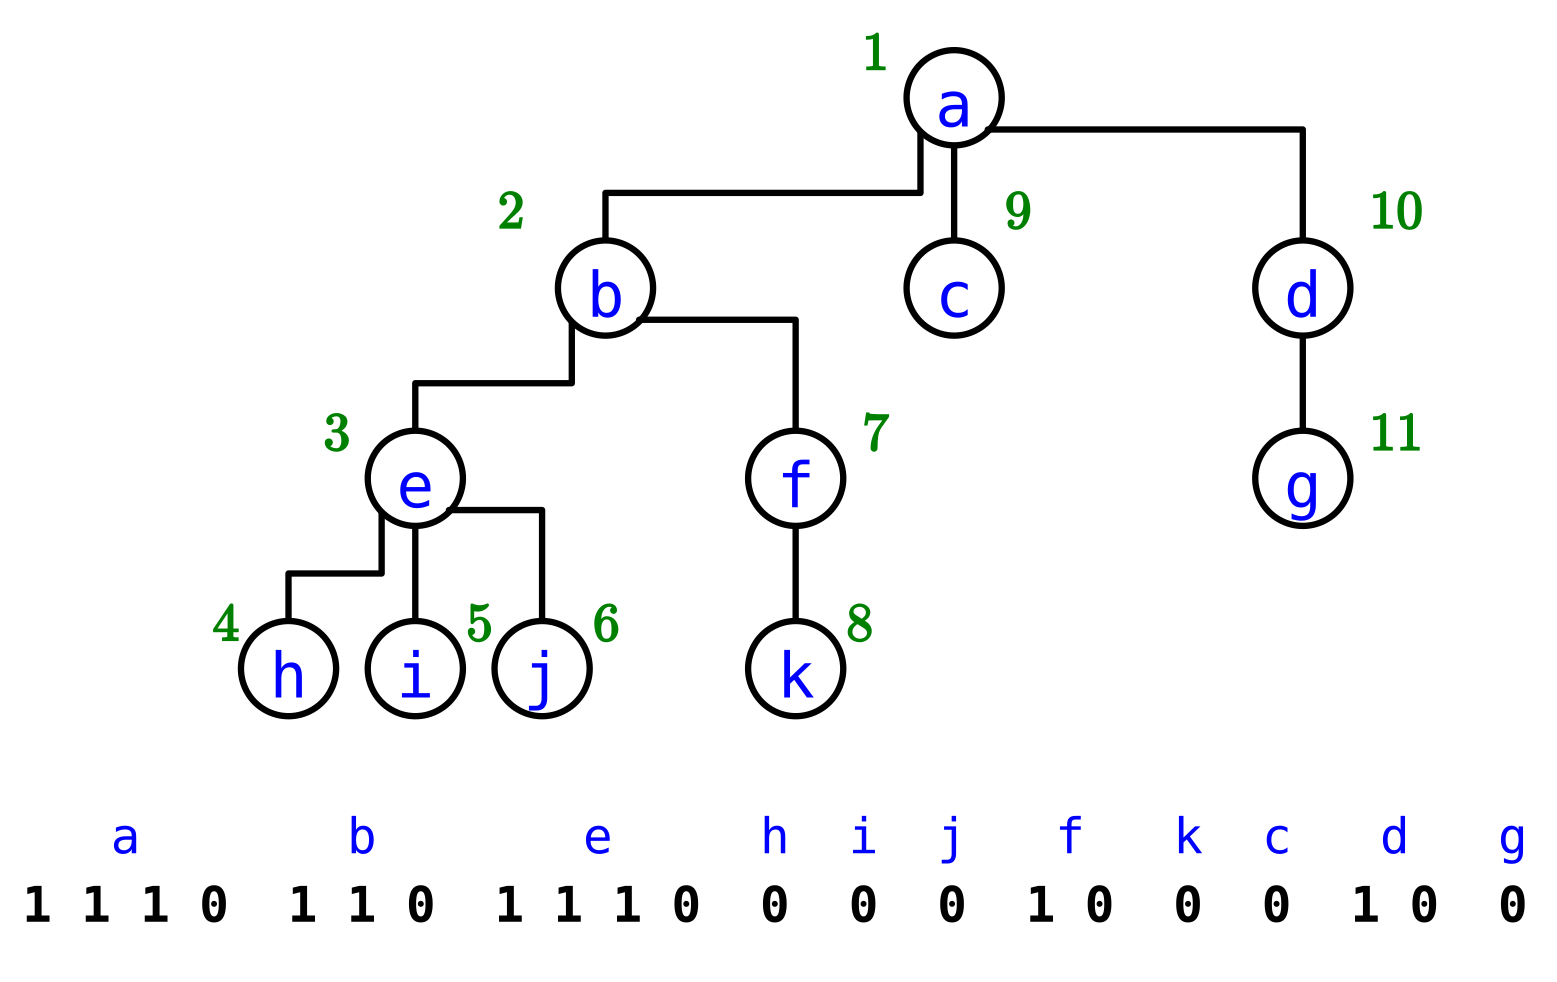
\includegraphics[width=0.8\linewidth]{ManziniDFUDS.png}
    \caption{Example of DFUDS (Depth-First Unary Degree Sequence) encoding of a rooted tree, adapted from Manzini~\cite{manzini2025succinct}.}
    \label{fig:dfuds_manzini}
\end{figure}

We base our succinct tree representation on the Depth-First Unary Degree Sequence (DFUDS) encoding introduced by Benoit et al.~\cite{benoit2005representing}. DFUDS encodes the topology of a rooted tree in $2n + o(n)$ bits while supporting key navigational queries—such as parent, $i$-th child, subtree size, and lowest common ancestor—in $O(1)$ time. This makes DFUDS an ideal foundation for succinct tree structures and for zipper-like navigation over large models. In our Haskell prototype, we store the DFUDS bitstring inside a \texttt{Poppy512} index from the \texttt{hw-rankselect} library, while the node payloads are stored contiguously in an unboxed vector. This clean separation between topology and payload is what allows us to approach the information-theoretic minimum for space and still obtain highly cache-friendly traversals.

\begin{remark}
    The following explanation is intentionally informal and focuses on intuition rather than full formalism.
\end{remark}

The encoding is as conceptually simple as efficient in practice. We traverse the tree in depth-first pre-order: starting from the root, we visit its first child and all of its descendants, then the second child, and so on. For every node with $d$ children, we append $d$ \texttt{1}s followed by a single \texttt{0} to a global bitstring. For example, in Figure~\ref{fig:dfuds_manzini}, the root node \textbf{a} has three children and contributes \texttt{1110}; node \textbf{b} has two children and contributes \texttt{110}; node \textbf{e} has three children and contributes \texttt{1110}; each leaf (such as \textbf{h}, \textbf{i}, or \textbf{j}) contributes a single \texttt{0}; and so on for the remaining nodes. Concatenating these local codes in the order of the traversal yields a single contiguous DFUDS bitstring that fully captures the parent–child structure of the original tree without storing any explicit pointers.

In practice, implementations often prepend one artificial \texttt{1} at the beginning of the DFUDS string. This ensures enables constant-time navigation via fast \texttt{rank} and \texttt{select} operations on the underlying bitvector. Future work \emph{could} explore complementing DFUDS (which is naturally depth-first) with LOUDS (Level-Order Unary Degree Sequence). 
Intuitively, LOUDS plays the same role as DFUDS but for breadth-first order: it provides a succinct encoding of the same tree topology, while arranging nodes in level order rather than depth-first order, enabling efficient BFS traversals within the same succinct framework.
